\documentclass{report}
\usepackage[francais]{babel}
\usepackage[utf8]{inputenc}
\usepackage[T1]{fontenc}
\usepackage{float}
\usepackage{amssymb}
\usepackage{stmaryrd}

\usepackage{graphicx}
\usepackage{subfig}

\makeatletter
\newcommand{\Spvek}[2][r]{%
  \gdef\@VORNE{1}
  \left(\hskip-\arraycolsep%
  \begin{array}{#1}\vekSp@lten{#2}\end{array}%
  \hskip-\arraycolsep\right)}

\def\vekSp@lten#1{\xvekSp@lten#1;vekL@stLine;}
\def\vekL@stLine{vekL@stLine}
\def\xvekSp@lten#1;{\def\temp{#1}%
  \ifx\temp\vekL@stLine
  \else
  \ifnum\@VORNE=1\gdef\@VORNE{0}
  \else\@arraycr\fi%
  #1%
  \expandafter\xvekSp@lten
  \fi}
\makeatother

\newcommand{\HRule}{\rule{\linewidth}{0.5mm}}
\bibliographystyle{unsrt}
\begin{document}

\begin{titlepage}

  \begin{center}

    \textsc{\LARGE Rapport}\\[1.5cm]

    \textsc{\Large EPITA}\\[0.5cm]

    \HRule \\[0.4cm]
           { \huge \bfseries Métaheuristiques pour l'optimisation difficile}\\[0.4cm]

           \HRule \\[1.5cm]

           \large
           \emph{Auteurs:}\\
           Loïc \textsc{Bethmont}\\
           Victor \textsc{Lenoir}\\

           \vfill

           % Bottom of the page
           {\large \today}

  \end{center}

\end{titlepage}
%\maketitle
\newpage
\tableofcontents
\newpage

\chapter{Introduction}

Une métaheuristique est un algorithme d'optimisation permettant de
résoudre des problèmes difficiles de manière simple.  Un problème est
dis difficile quand il est inconcevable de parcourir la totalité de
l'espace de solutions pour trouver l'optimum global.


Les métaheuristiques sont des algorithmes très géneraux et avec un
haut niveau d'abstraction et peuvent par conséquent être appliquées sur
un grand nombre de problèmes différents.


Ce sont géneralement des méthodes stochastiques itératives qui tentent
de converger vers un optimum global.


Les métaheuristiques sont très utilisées lorsqu'un problème est trop
complexe pour obtenir une solution analytique ou une autre solution
algorithmique ou lorsqu'une solution alternative est trop coûteuse ou
encore lorsqu'on ne connaît pas de méthodes pour résoudre le problème.

\chapter{Algorithmes}

\section{Recuit simulé}
%Parle vite fais que c'est une methode qui nous vient de la
%metallurgie, j'y fais reference apres
\subsection{Benchmarks}

\section{Programmation génétique}

Tout comme le recuit simulé, la programmation génétique est une
métaheuristique inspirée d'un autre mécanisme : la sélection
naturelle, expliqué par Charles Darwin.

La sélection naturelle explique l'adaptation des espèces à leur
environnement au fil des génerations. Son principe est simple et
explique que les caractéristiques favorisant la survie/reproduction
d'un individu augmentent en fréquence car l'individu aura plus
tendance à se reproduire/survivre et par conséquent avoir des
descendants et les descendants auront eux aussi cette même
caractéristique favorable à la survie.\\\\

La programmation génétique fonctionne de la même manière, on va
modéliser notre problème de la même manière en utilisant le même
vocabulaire: reproduction, individu, population, séléction.\\\\

La fonction à maximiser/minimiser est appelée fonction de fitness et
indique si un individu "fit"/est adapté à son environnement.\\\\

Le principe de l'algorithme est simple:
\begin{enumerate}
\item Initialisation aléatoire d'une population
\item Reproduction de la population : cross-over, mutation
\item \'Evaluation de fitness pour chaque individu de la population
\item Sélection des individus les plus adaptés (ayant la fitness la plus élevé)
\item Répeter étape 2,3,4 jusqu'à convergence
\end{enumerate}

Il faut noter que même si la programmation génétique est une méthode
de résolution très abstraite, elle nécessite un certain nombre de
paramètres : la taille de la population initial, le nombre de
cross-over/mutation, le nombre d'individus sélectionnés à l'étape 4.
De plus il faut noter que tout comme dans la sélection naturelle, la
mutation est primordiale à l'évolution, en effet elle permet
d'introduire de nouvelles caractéristiques dans une population. Sans
celà on ne ferait que des combinaisons de caractéristiques déjà
existantes.

\subsection{Benchmarks}

Les benchmarks de la programmation génétique ont été réalisé sur des
fonctions à minimiser. Les minimums globaux de cette fonction sont
connus et ainsi on pourra vérifier que le minimum global est
atteint.\\ Ci-dessous la fonction Schwefel de la forme:
$$SH(x) = \sum_{i=1}^{n}{-x_i\sin{(\sqrt{\mid{}x_i\mid{}})}}$$ Un
individu est caracterisé par ses gènes, ici ce sont les $x_i$.  La
figure \ref{geneticschwefel} montre ici l'évolution de la fonction de
Schwefel à 10 variables/gènes au fil des génerations. On observe que
l'algorithme converge bien vers le minimum global connu qui est de
-4189.829.
\begin{figure}[H]
  \centering
  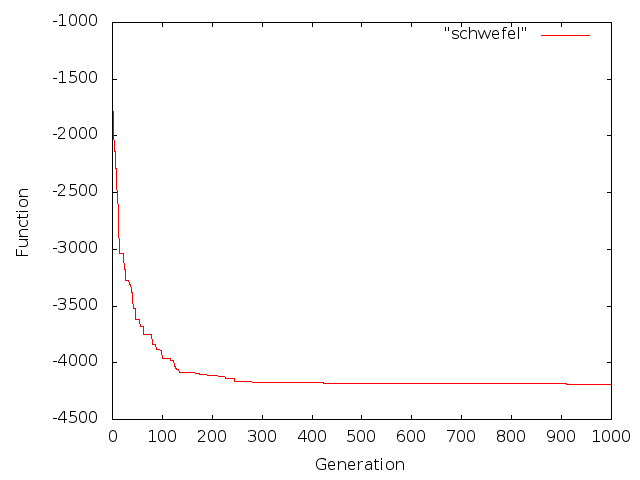
\includegraphics[width=300px]{genetic_schwefel.png}
  \caption{Minimum de la fonction de Schwefel au fil des génerations}
  \label{geneticschwefel}
\end{figure}

On peut observer que la convergence est rapide même si la population
était seulement de 100 individus et que chaque individus avait 10
gènes.

\chapter{Conclusion}

\end{document}
